\section{Exercise 1}

Consider the one-dimensional Laplace equation
\begin{equation*}
u_{xx} = f(x) \qquad (0 < x < 1)
\end{equation*}
with the source term $f(x) = x + \cos(2 \pi x)$, subject to different kinds of boundary conditions
\begin{equation*}
\begin{aligned}
u(0) &= a, &\quad u(1) &= b &\qquad& \text{(Dirichlet-Dirichlet)} \\
u_x(0) &= a, &\quad u_x(1) &= b &\qquad& \text{(Neumann-Neumann)} \\
u(0) &= a, &\quad u_x(1) &= b &\qquad& \text{(Dirichlet-Neumann)}. \\
\end{aligned}
\end{equation*}

An analytical solution is
\begin{equation*}
u(x) = C_1 + C_2 x + \frac{1}{6}x^3 - \frac{1}{4 \pi^2}\cos(2 \pi x)),
\end{equation*}
where the constants $C_1$ and $C_2$ are determined from two boundary conditions.
Note that when Neumann-Neumann boundary conditions are imposed, $C_1$ is undetermined and so the solution is determined only up to a constant.

Grid:
\begin{center}
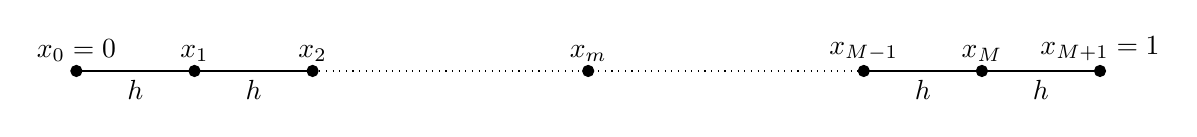
\begin{tikzpicture}
\draw (0,0) -- (3,0);
\draw[dotted] (3,0) -- (10,0);
\draw (10,0) -- (13,0);
\filldraw (0.0,0) circle (2pt) node[anchor=south] {$x_0 = 0$};
\filldraw (1.5,0) circle (2pt) node[anchor=south] {$x_1$};
\filldraw (3.0,0) circle (2pt) node[anchor=south] {$x_2$};
\filldraw (6.5,0) circle (2pt) node[anchor=south] {$x_m$};
\filldraw (10.0,0) circle (2pt) node[anchor=south] {$x_{M-1}$};
\filldraw (11.5,0) circle (2pt) node[anchor=south] {$x_{M}$};
\filldraw (13.0,0) circle (2pt) node[anchor=south] {$x_{M+1} = 1$};
\node[anchor=north] at (0.75, 0) {$h$};
\node[anchor=north] at (2.25, 0) {$h$};
\node[anchor=north] at (10.75, 0) {$h$};
\node[anchor=north] at (12.25, 0) {$h$};
\end{tikzpicture}
\end{center}

Inner points:
\begin{equation*}
\frac{U_{m+1} - 2 U_m + U_{m-1}}{h^2} = f(x_m)
\end{equation*}
Dirichlet, left:
\begin{equation*}
u(0) = U_0
\end{equation*}
Von-Neumann, left, 2nd order:
\begin{equation*}
u_x(0) \approx -\frac{(3/2)U_0 -2U_1 + (1/2)U_2}{h}
\end{equation*}

Discretized equation:
\begin{equation*}
\renewcommand{\arraystretch}{2.8} % stretch matrix vertically to make it square
\begin{bmatrix}
-2/h^2 & +1/h^2  & 0 & \cdots & 0 \\
+1/h^2  & -2/h^2 & +1/h^2  & \ddots & \vdots \\
0 & \ddots & \ddots & \ddots & 0 \\
\vdots & \ddots & +1/h^2 & -2/h^2 & +1/h^2\\
0 & \cdots & -1/2h & +2/h & -3/2h  \\
\end{bmatrix}
\begin{bmatrix}
U_1 \\ U_2 \\ \vdots \\ U_M \\ U_{M+1} \\
\end{bmatrix}
=
\begin{bmatrix}
f(x_1) - \alpha/h^2 \\ f(x_2) \\ \vdots \\ f(x_M) \\ \sigma \\
\end{bmatrix}
\end{equation*}

% This file was created by tikzplotlib v0.9.6.
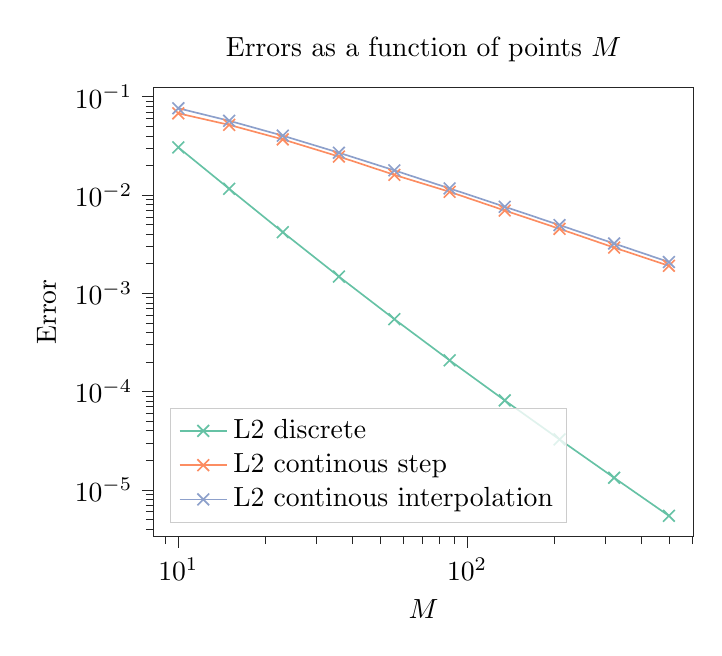
\begin{tikzpicture}

\definecolor{color0}{rgb}{0.4,0.76078431372549,0.647058823529412}
\definecolor{color1}{rgb}{0.988235294117647,0.552941176470588,0.384313725490196}
\definecolor{color2}{rgb}{0.552941176470588,0.627450980392157,0.796078431372549}

\begin{axis}[
axis line style={white!15!black},
legend cell align={left},
legend style={fill opacity=0.8, draw opacity=1, text opacity=1, at={(0.03,0.03)}, anchor=south west, draw=white!80!black},
log basis x={10},
log basis y={10},
tick align=outside,
tick pos=left,
title={Errors as a function of points \(\displaystyle M\)},
x grid style={white!80!black},
xlabel={\(\displaystyle M\)},
xmin=8.22340159426889, xmax=608.020895329329,
xmode=log,
xtick style={color=white!15!black},
y grid style={white!80!black},
ylabel={Error},
ymin=3.36937677353097e-06, ymax=0.123149403927534,
ymode=log,
ytick style={color=white!15!black}
]
\addplot [semithick, color0, mark=x, mark size=3, mark options={solid}]
table {%
10 0.0305423931057193
15 0.0115681562237246
23 0.00418684706084268
36 0.00147778708799188
56 0.000545344047314135
87 0.000207740833940065
135 8.12810709689553e-05
209 3.25522318966553e-05
323 1.32584662173129e-05
500 5.43191966701882e-06
};
\addlegendentry{L2 discrete}
\addplot [semithick, color1, mark=x, mark size=3, mark options={solid}]
table {%
10 0.0678018959630194
15 0.0517494504008614
23 0.0368263735747522
36 0.0246290794091911
56 0.016038328828533
87 0.0107798628521512
135 0.00695920086265971
209 0.00453050481902805
323 0.00291728074872839
500 0.00190428788556582
};
\addlegendentry{L2 continous step}
\addplot [semithick, color2, mark=x, mark size=3, mark options={solid}]
table {%
10 0.0763886004771024
15 0.0569765338780135
23 0.0401712964166644
36 0.0269473845612725
56 0.0178234215050096
87 0.0116718071194704
135 0.00760171372836376
209 0.00494277609000366
323 0.00321158725355576
500 0.00208024898986026
};
\addlegendentry{L2 continous interpolation}
\end{axis}

\end{tikzpicture}

